% Section 3.7 — paste into the body of the MDPI manuscript.
% Requires graphicx (normally loaded by the MDPI class).
% Place convergence_4datasets_8panels.pdf beside the main .tex file.
\subsection{Convergence and Population Diversity Analysis}
\label{subsec:convergence_diversity}

To further investigate the evolutionary behavior of the proposed crossover operators, a convergence and population diversity analysis was conducted on four representative classification datasets: Dermatology, Ionosphere, Spambase, and Vehicle. These datasets include binary and multiclass classification problems, allowing the crossover strategies to be examined under different chromosome structures. Each configuration was evaluated over 30 independent runs using a fixed budget of 100,000 fitness evaluations.

Population diversity was quantified using the normalized average pairwise Hamming distance between chromosomes. This measure expresses the proportion of differing codon positions across pairs of individuals in the population. Higher values indicate greater genotypic diversity, whereas lower values indicate increasing population homogeneity. The convergence curves show the mean best-so-far fitness, and the diversity curves show the mean population diversity. Shaded regions indicate one standard deviation around the mean.

Figure~\ref{fig:convergence_diversity} presents the convergence and diversity trajectories for all four datasets. The left column shows best-so-far fitness against the number of fitness evaluations; the right column shows normalized population diversity. Since the fixed evaluation budget may interrupt the final generation, the diversity curves are restricted to evaluation ranges with observations from all 30 runs for each operator, avoiding comparisons based on unequal sample counts.

On Dermatology, TargetedWorst exhibits relatively rapid initial fitness improvements. Both targeted variants maintain greater population diversity than Standard over substantial portions of the search. At 60,000 fitness evaluations, the diversity differences between Standard and Targeted and between Standard and TargetedWorst are statistically significant (Holm-adjusted Wilcoxon $p=3.18\times10^{-5}$ and $p=9.94\times10^{-5}$, respectively). No statistically significant diversity difference was observed between the two targeted variants. Although TargetedWorst obtained the best mean final fitness in this experiment, pairwise tests did not identify statistically significant differences in final fitness.

On Ionosphere, Targeted achieves significantly better final fitness than Standard. The recorded convergence and diversity trajectories of Targeted and TargetedWorst coincide. On Spambase, the targeted variants maintain greater population diversity than Standard over substantial portions of the search, but the final-fitness difference between Standard and Targeted is not statistically significant. The two targeted variants again exhibit identical recorded trajectories.

Vehicle provides a multiclass case in which the targeted variants generally maintain greater genotypic diversity than Standard, while the observed final-fitness difference between Standard and Targeted is not statistically significant. Thus, increased diversity does not necessarily translate into better final optimization performance under the available evaluation budget.

An implementation-specific characteristic explains the identical behavior of Targeted and TargetedWorst observed on the binary datasets. For a problem with $C$ classes, the chromosome contains $C-1$ explicit classification rules, with the remaining class represented by the default branch. TargetedWorst restricts crossover positions to the segment corresponding to the worst-performing class, except when that class is the default class, in which case the entire chromosome is considered. When $C=2$, the single explicit-rule segment already spans the entire chromosome. Therefore, the class-specific restriction is ineffective for either possible worst-performing class, and TargetedWorst can select the same candidate crossover positions as Targeted. With otherwise equivalent selection and exchange operations and the same random seed, the operators can follow identical evolutionary trajectories, as observed on Ionosphere and Spambase.

Overall, Figure~\ref{fig:convergence_diversity} indicates that the targeted crossover variants often preserve greater genotypic diversity, particularly on Dermatology, Spambase, and Vehicle, without consistently producing statistically significant improvements in final fitness. The effects are dataset-dependent. Furthermore, higher genotypic diversity should not be interpreted as direct evidence of improved generalization performance or a causal explanation for differences in classification accuracy.

\begin{figure}[htbp]
\centering
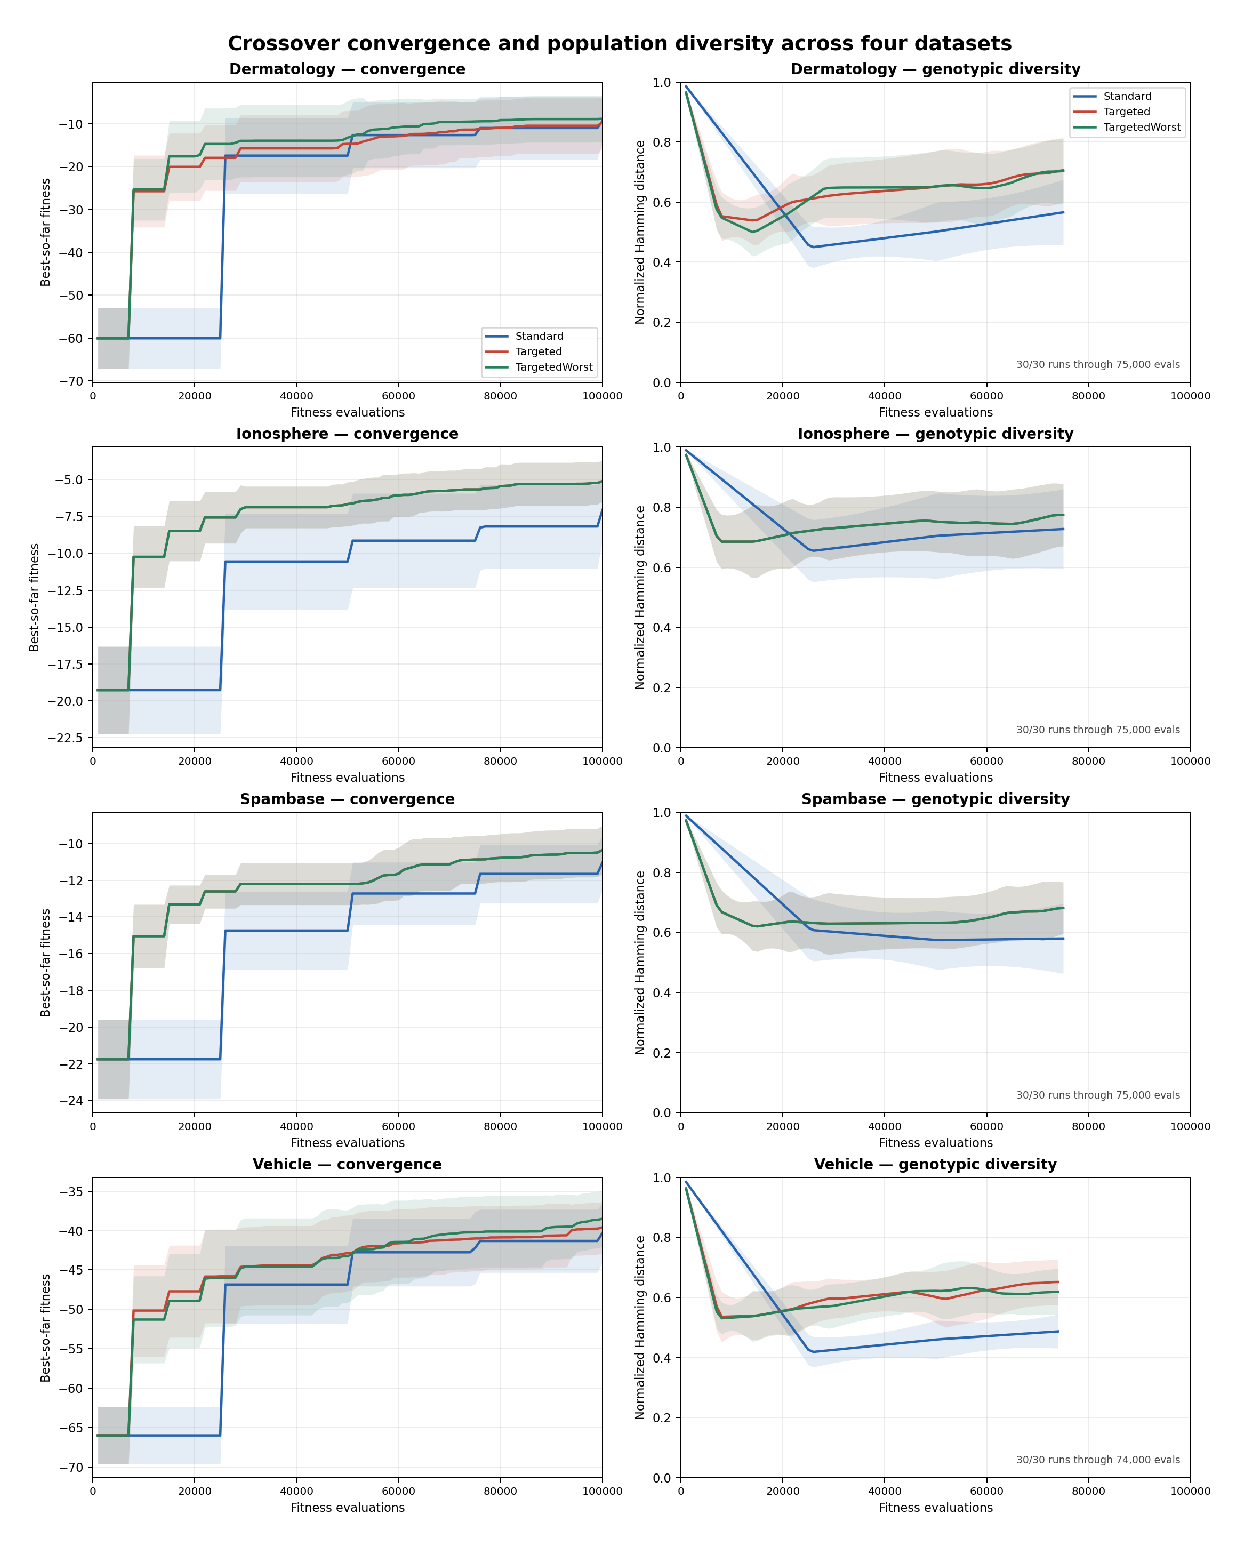
\includegraphics[width=\textwidth]{convergence_4datasets_8panels.pdf}
\caption{Convergence and population diversity of the Standard, Targeted, and TargetedWorst crossover operators on Dermatology, Ionosphere, Spambase, and Vehicle. The left column presents mean best-so-far fitness, while the right column presents mean normalized average pairwise Hamming distance. Results are aggregated over 30 independent runs per operator. Shaded regions represent the mean $\pm$ one standard deviation. Diversity curves are restricted to evaluation ranges with complete observations across all runs, whereas convergence curves extend to the fixed budget of 100,000 fitness evaluations.}
\label{fig:convergence_diversity}
\end{figure}
